
%(BEGIN_QUESTION)
% Copyright 2009, Tony R. Kuphaldt, released under the Creative Commons Attribution License (v 1.0)
% This means you may do almost anything with this work of mine, so long as you give me proper credit

This fluid diagram shows the components and connections of a Bettis self-contained hydraulic module used to automatically shut off a ``line valve'' on a natural gas pipeline in the event of the pipeline pressure going outside of its limits (either falling below the low-pressure limit or rising above the high-pressure limit):

$$\includegraphics[width=15.5cm]{i01722x01.eps}$$

Circle the appropriate box in each of the ``multi-box'' symbols for the Pressure pilot, Solenoid trip, Auto/Man, and Reset spool valve mechanisms showing their respective positions {\it during typical operation, when the line valve is supposed to be open and pipeline pressure is within normal operating limits}.

Identify the effect of a loose hydraulic tube fitting connection between the Solenoid trip spool valve and the hydraulic reservoir, as the line valve is in normal operation (open).  Will this loose fitting cause the line valve to fail closed or not?  Explain your answer.

\underbar{file i01722}
%(END_QUESTION)





%(BEGIN_ANSWER)

1 points for each correctly-circled box, 3 points for the correct ``trip'' answer, and 3 points for correct reasoning:

$$\includegraphics[width=15.5cm]{i01722x02.eps}$$

A loose fitting between any spool valve and the reservoir will {\bf not} cause the line valve to go to its fail position.

\vskip 10pt

The reason a loose fitting between any spool valve and the reservoir will not trip the line valve is because these lines are not pressurized while the line valve is open.  In the event of a trip at that spool valve (with the loose fitting), the worse that could happen is a little bit of hydraulic fluid dripping out the loose fitting.

%(END_ANSWER)





%(BEGIN_NOTES)

{\bf This question is intended for exams only and not worksheets!}.

%(END_NOTES)


